% -------------------- Information --------------------

\newcommand{\TITLE}{Features of Portable Document Format}
\newcommand{\AUTHOR}{Jason Chen}
\newcommand{\SUBJECT}{Public Speaking}
\newcommand{\KEYWORDS}{}
\newcommand{\INSTITUTE}{School of Mathematical Sciences, Tongji University}

% -------------------- Packages --------------------

\documentclass[xcolor=dvipsnames]{beamer}
\usepackage{amsmath}
% \usepackage{amsthm} % loaded by beamer.
\usepackage{amssymb}
\usepackage{commath} % abs, norm
\usepackage[mathscr]{euscript}
\usepackage{float} % 你们这帮float给我乖乖听话 HHHHHHHHHHH.
\usepackage{fontspec}
\usepackage{graphicx}
% \usepackage{hyperref} % loaded by beamer.
\usepackage{mathtools} % \xleftrightarrow.
\usepackage[timeinterval=1, font=Times, resetatpages=2]{tdclock}
\usepackage[absolute, overlay]{textpos}
\usepackage{tikz}
\usepackage{ulem} % strikethrough \sout
% \usepackage{xcolor} % loaded by beamer.
\usepackage[printwatermark]{xwatermark} % Foreground Watermarks.
\usepackage[all, cmtip]{xy}

% -------------------- Settings --------------------

% Package: beamer

\transpush<2>[duration=2]
\usetheme{Berlin}

% Package: graphicx

\graphicspath{{resources/}} % 图像文件目录

% Package: hyperref

\hypersetup{
    linktoc             =   all,
    colorlinks          =   true,
    linkcolor           =   cyan,
    anchorcolor         =   black,
    citecolor           =   green,
    filecolor           =   cyan,
    menucolor           =   red,
    runcolor            =   filecolor,
    urlcolor            =   magenta,
    pdftitle           	=   {\TITLE},
    pdfauthor          	=   {\AUTHOR},
    pdfsubject         	=   {\SUBJECT},
    pdfcreator			=	{Visual Studio Code},
    pdfproducer			=	{XeLaTeX with documentclass beamer},
    pdfkeywords        	=   {\KEYWORDS},
    bookmarksnumbered   =   true,
    pdfstartview        =   Fit,
    pdfpagelayout       =   OneColumn,
    pdfpagemode			=   FullScreen
}

% Package: tdclock

\newcommand{\FrameTextCrono}[1]{
    \begin{textblock*}{\paperwidth}(\textwidth + 1em, \textheight + 1em)
        #1
    \end{textblock*}
}

\newcommand{\FrameTextResetCrono}[1]{
    \begin{textblock*}{\paperwidth}(\textwidth + 1.5em, \textheight - 0.5em)
        #1
    \end{textblock*}
}

\newcommand{\ResetCronoBox}{\resetcrono{\fbox{reset}}}

\let\oldframe\frame
\let\oldendframe\endframe
\renewenvironment{frame}
    {\oldframe\FrameTextCrono{\small\color{blue}{\crono}}}
    {\oldendframe}

\let\oldtitlepage\titlepage
\renewcommand{\titlepage}{\oldtitlepage\FrameTextResetCrono{\ResetCronoBox}}

% Package: xwatermark

\newsavebox\mybox
\savebox\mybox{\tikz[color=cyan, opacity=0.2]\node{\fontspec{Comic Sans MS}\SUBJECT};}
\newwatermark*[
    allpages,
    angle=45,
    scale=3,
    xpos=0,
    ypos=0
]{\usebox\mybox}

% Title

\title{\TITLE}
\author{\AUTHOR}
\date{\tdyear\dateseparator\tdmonth\dateseparator\tdday\hspace{1em}\tdtime}
\institute{\INSTITUTE}
\titlegraphic{
\includegraphics[width=0.1\paperwidth]{tongji.jpg}}

% Theorem Environments

\let\note\undefined
\newtheorem{note}{Note}[section]

% -------------------- General new commands --------------------

\DeclareMathAlphabet{\mathsfsl}{OT1}{cmss}{m}{sl}

% Expectation

\newcommand{\expect}{\operatorname{E}\expectarg}
\DeclarePairedDelimiterX{\expectarg}[1]{(}{)}{
  \ifnum\currentgrouptype=16 \else\begingroup\fi
  \activatebar#1
  \ifnum\currentgrouptype=16 \else\endgroup\fi
}

\newcommand{\innermid}{\nonscript\;\delimsize\vert\nonscript\;}
\newcommand{\activatebar}{
  \begingroup\lccode`\~=`\|
  \lowercase{\endgroup\let~}\innermid
  \mathcode`|=\string"8000
}

\newcommand{\diff}{\mathop{}\!\mathrm{d}}
\newcommand{\matr}[1]{\ensuremath{\mathsfsl{#1}}} % italic sans serif
\newcommand{\me}{\mathrm{e}}
\newcommand{\mi}{\mathrm{i}}
\newcommand{\restrict[1]}{\raisebox{-.5ex}{$|$}_{#1}}
\newcommand{\vect}[1]{\bm{#1}}

% -------------------- Specific new commands --------------------



% -------------------- Document --------------------

\begin{document}

    % -------------------- Title Page --------------------

    \begin{frame}
        \initclock
        \titlepage
        \pagenumbering{arabic}
    \end{frame}

    % -------------------- Contents --------------------

    \begin{frame}
        \frametitle{Contents}
        \tableofcontents
    \end{frame}

    % -------------------- Body --------------------

    \section{Introduction}

    \begin{frame}
        \frametitle{Background}
        \begin{itemize}
            \item PDF format was developed by Adobe in 1990s
                to present documents, including texts and images.
            \item Motivation.
        \end{itemize}
    \end{frame}

    \section{Feature I: Presenting Static Documents}

    \begin{frame}
        \frametitle{Presenting Static Documents}
        PDF format
        \begin{itemize}
            \item is wildly used.
            \item presents documents in a manner independent of environment.
        \end{itemize}
    \end{frame}

    \begin{frame}
        \frametitle{Preserving Typesetting}
        PDF files keep typesetting of documents.
        \begin{itemize}
            \item Texts, images and tables in PDF files will keep their positions
                so that the document looks the same
                whenever the application software, hardware,
                and operating systems are changed.
            \item \sout{PPT}.
        \end{itemize}
    \end{frame}

    \begin{frame}
        \frametitle{Preserving Typesetting (Continued)}
        A fake example. (Hot Pot?)
        \centering
        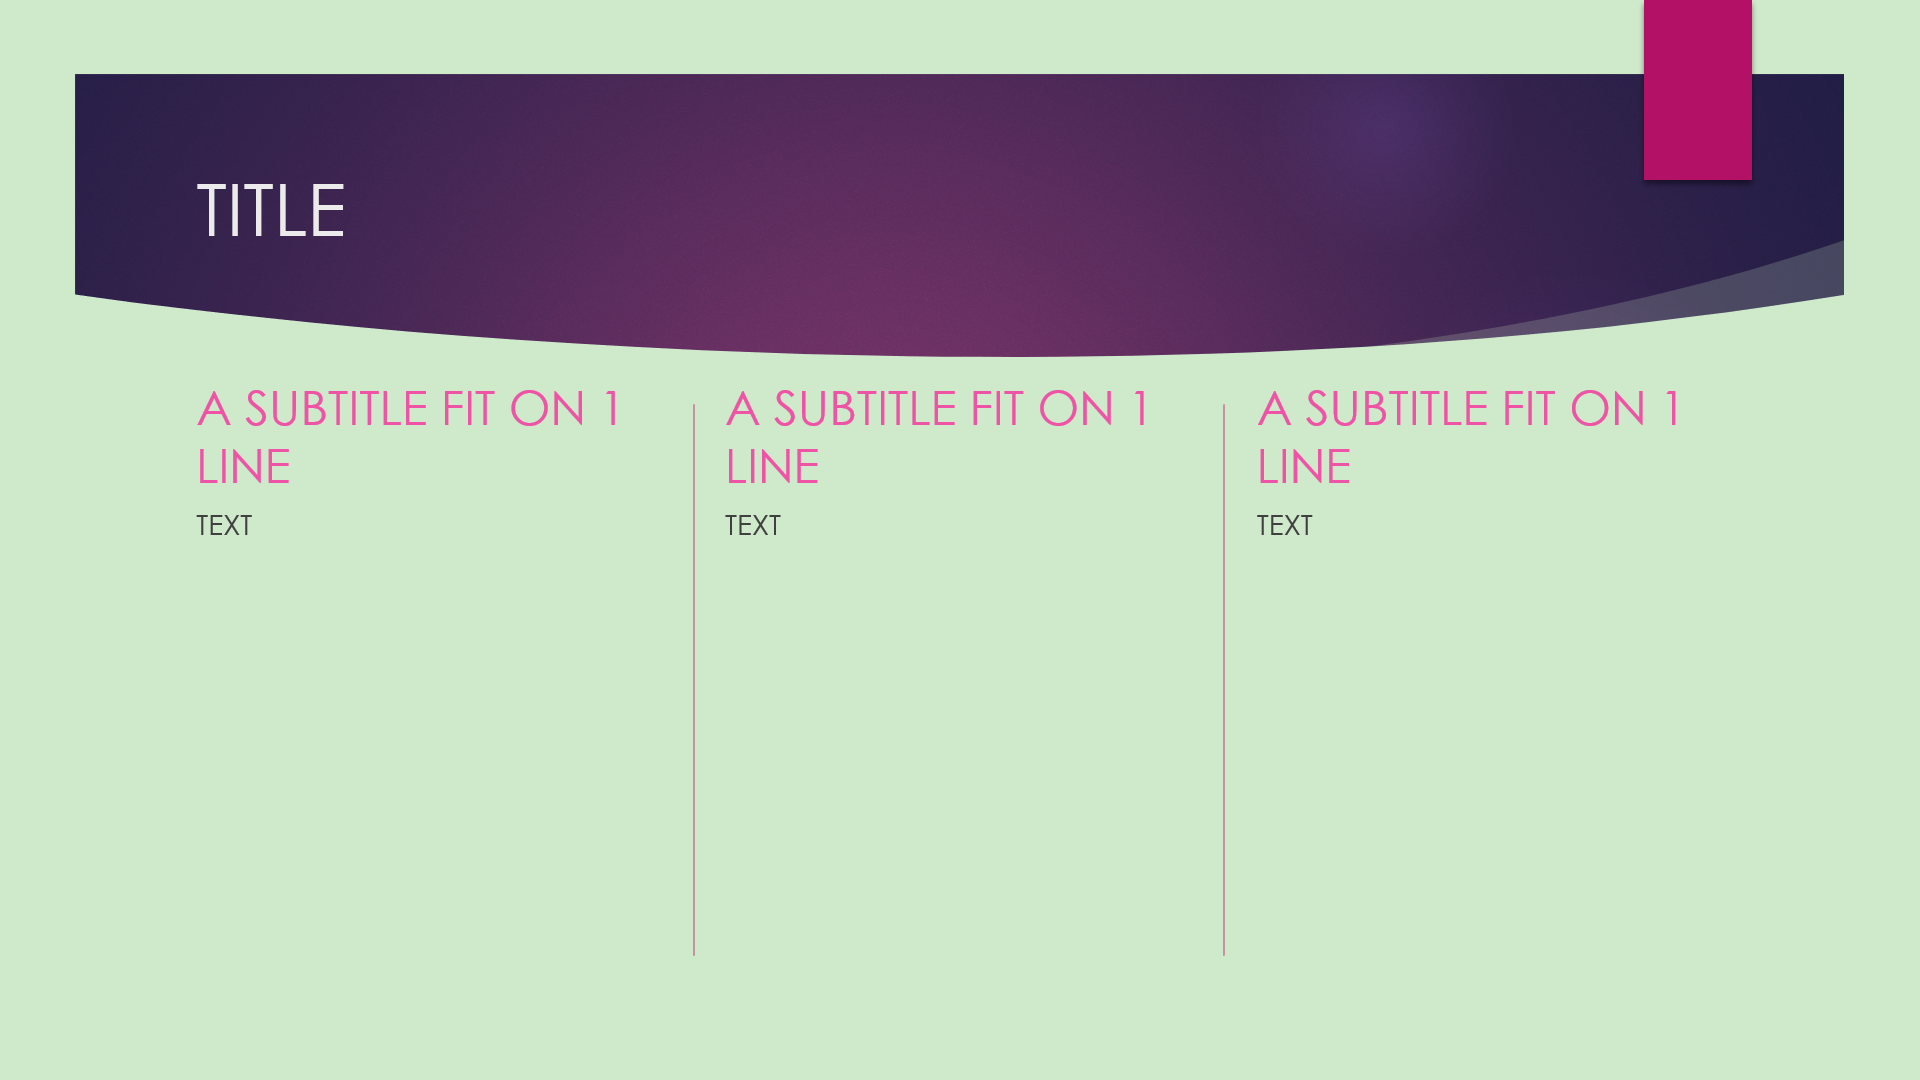
\includegraphics[scale=0.2]{fake_ppt.png}
    \end{frame}

    \begin{frame}
        \frametitle{Containing All Needed Files}
        PDF files contains all files needed to present the documents.
        \begin{itemize}
            \item e.g. font files.
            \item {\fontspec{Berlin Sans FB Demi}Berlin Sans FB Demi,}
            {\fontspec{Bradley Hand ITC}Bradley Hand ITC,}
            {\fontspec{Colonna MT}Colonna MT,}
            {\fontspec{Curlz MT}Curlz MT,}
            {\fontspec{Edwardian Script ITC}Edwardian Script ITC,}
            {\fontspec{Euclid Fraktur}Euclid Fraktur,}
            {\fontspec{Forte}Forte,}
            {\fontspec{Freestyle Script}Freestyle Script,}
            {\fontspec{Harlow Solid Italic}Harlow Solid Italic,}
            {\fontspec{Mistral}Mistral,}
            {\fontspec{Snap ITC}Snap ITC.}
        \end{itemize}
    \end{frame}

    \begin{frame}
        \frametitle{Containing All Needed Files (Continued)}
        A screenshot of previous page opened by my iPad's default viewer.
        \centering
        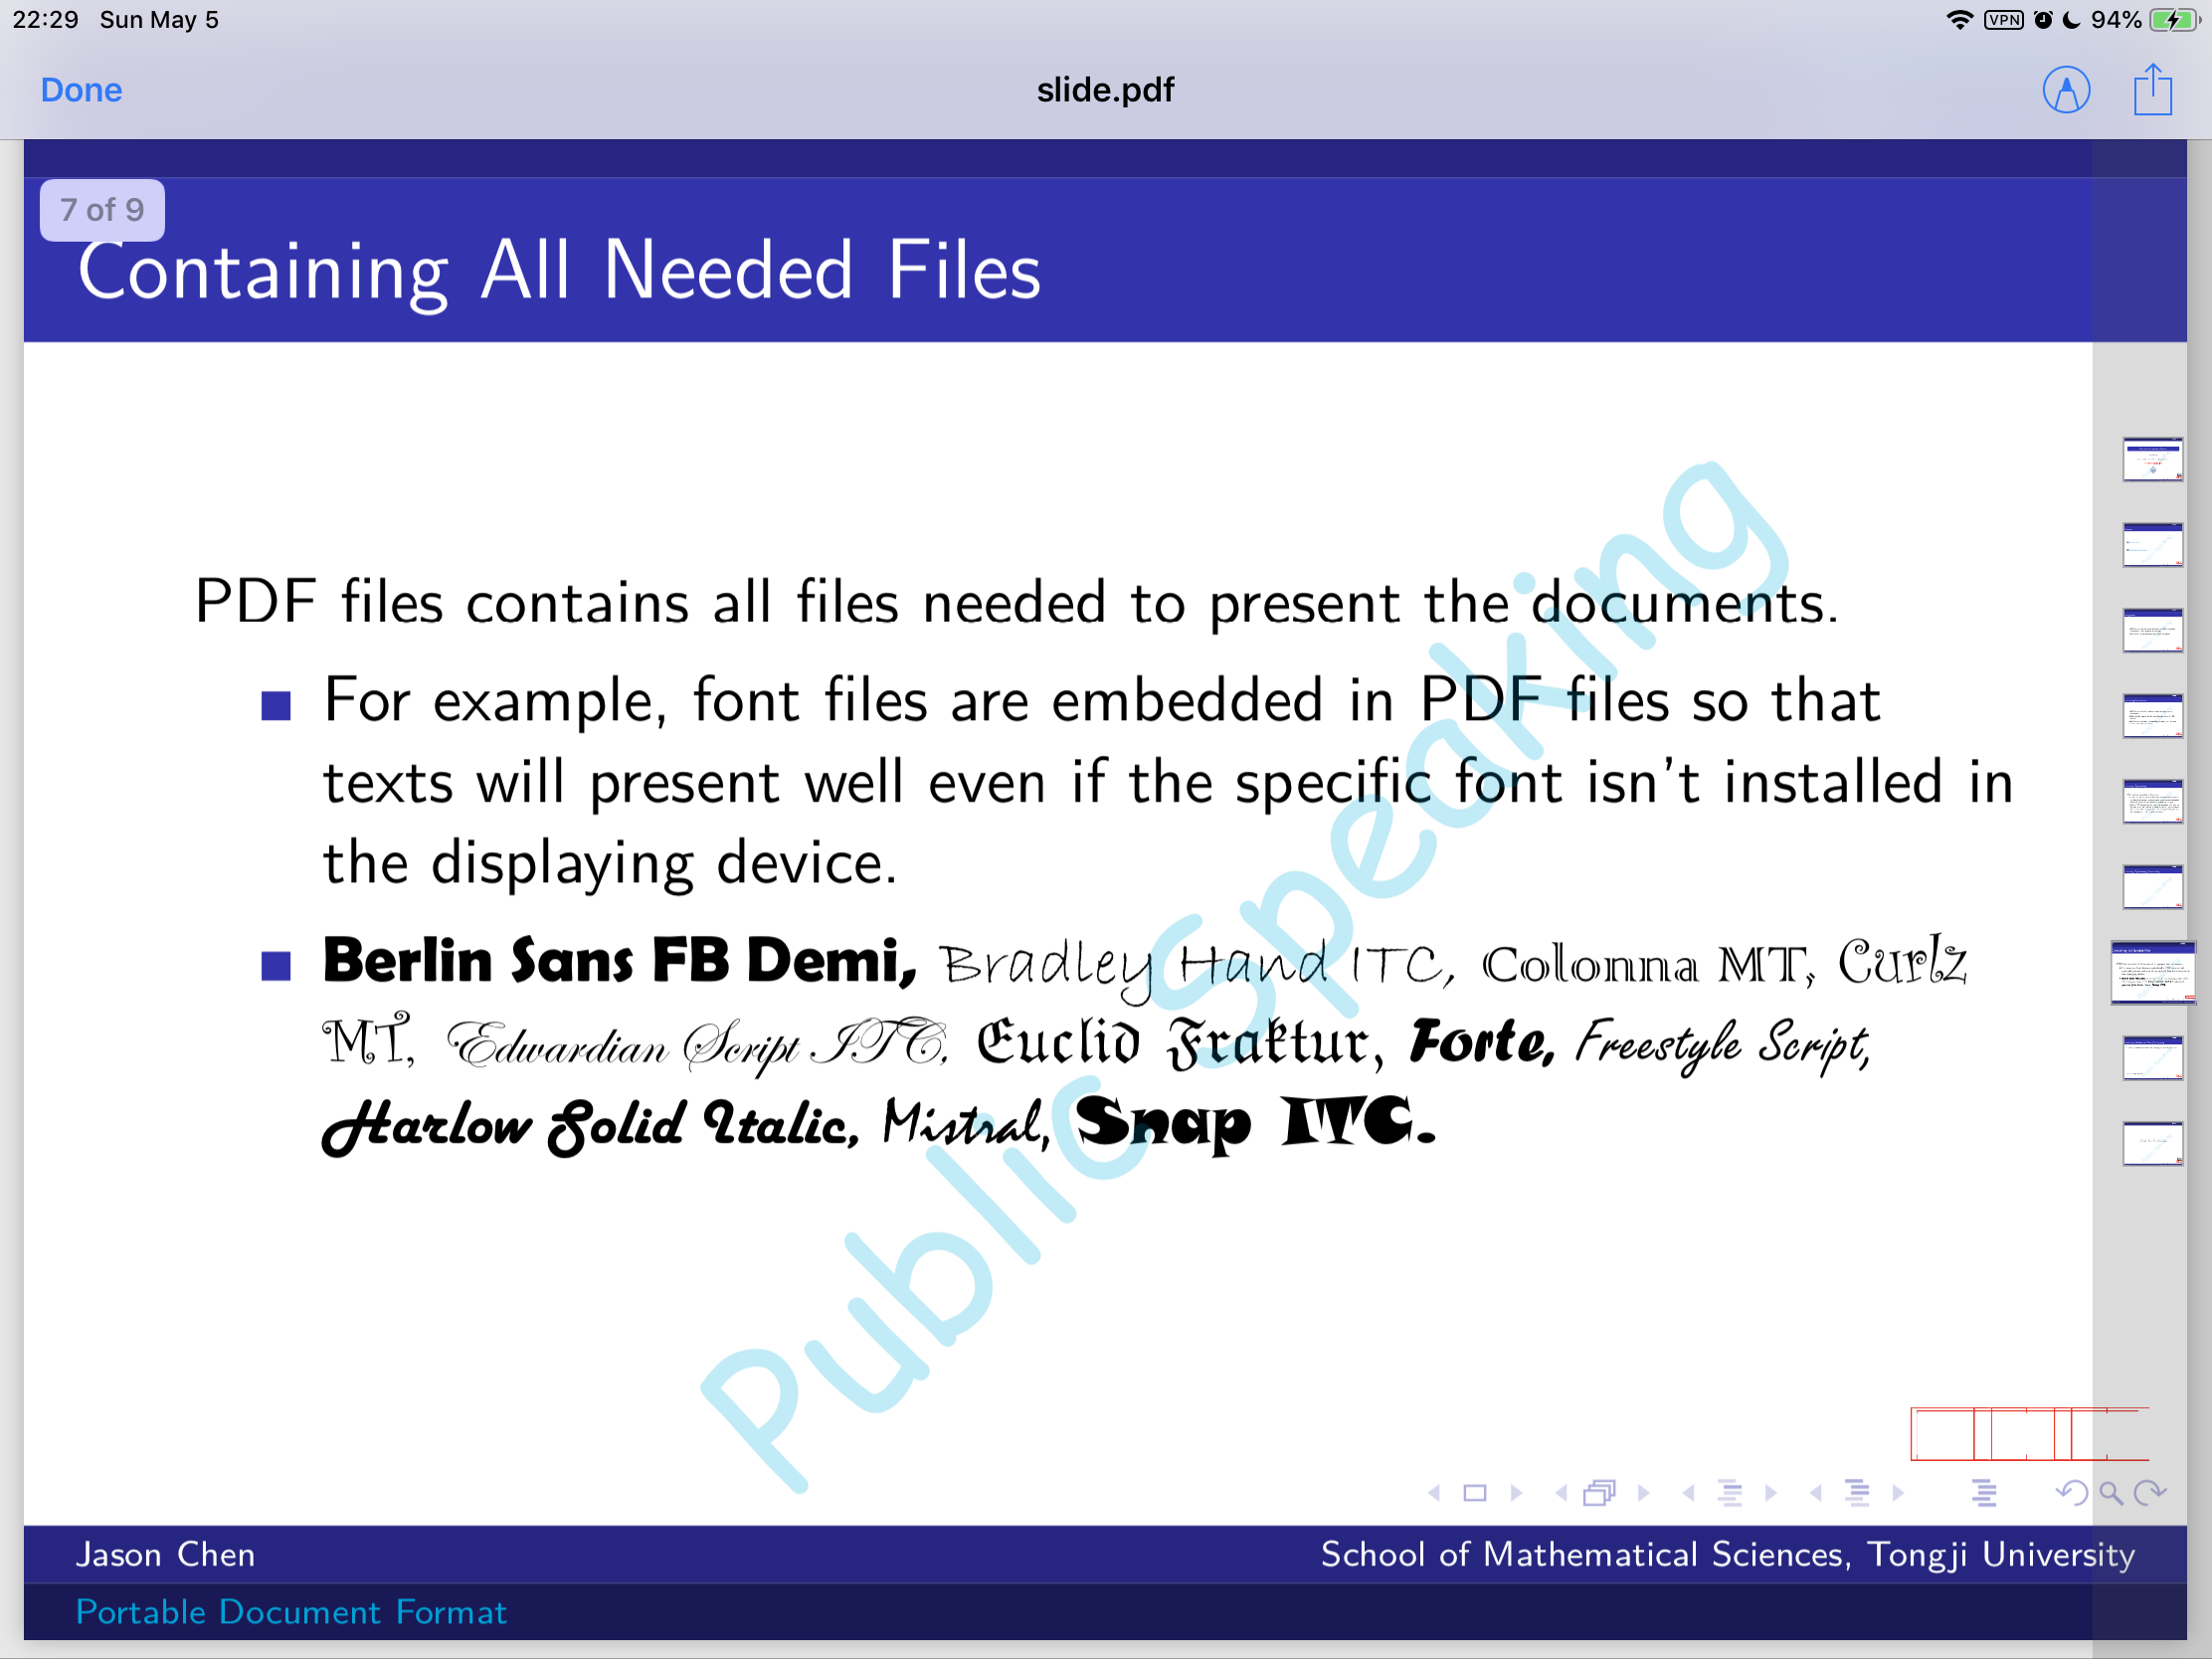
\includegraphics[scale=0.09]{fonts.png}
    \end{frame}

    \begin{frame}
        \frametitle{Containing All Needed Files (Continued)}
        A screenshot of our lecture ppt opened by Keynote on my iPad.
        \centering
        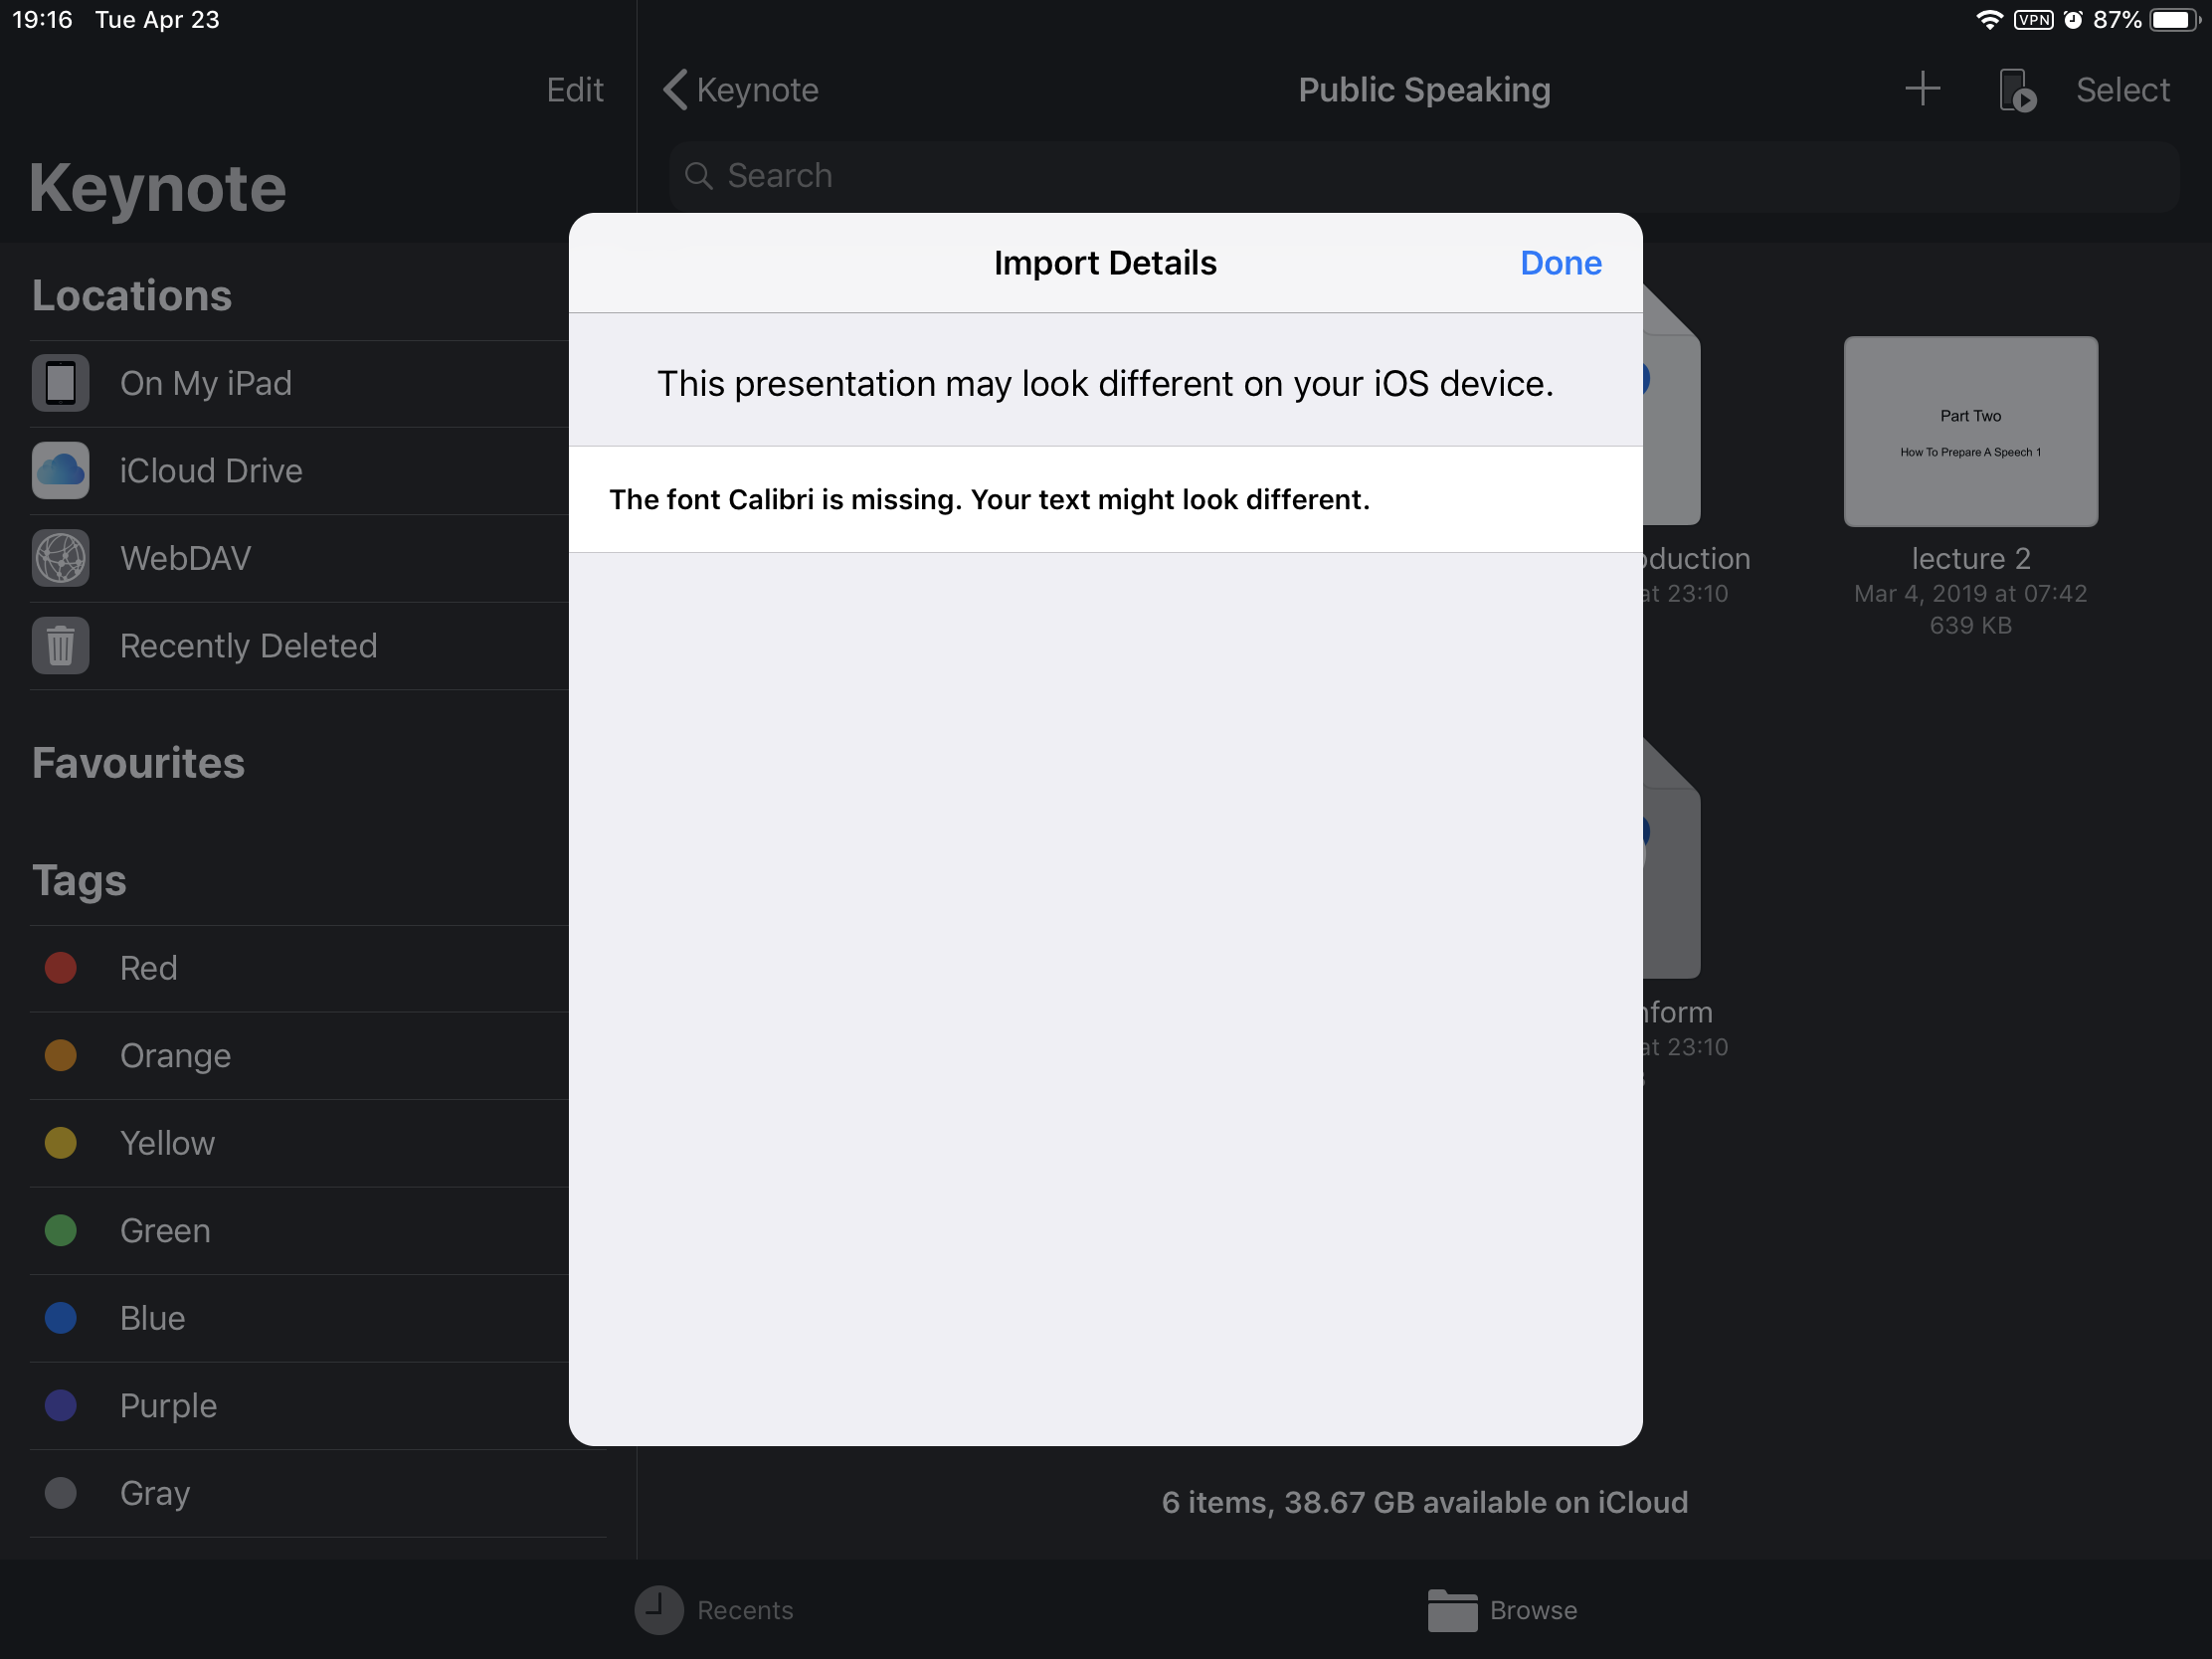
\includegraphics[scale=0.09]{missing_fonts.png}
    \end{frame}

    \section{Feature II: Presenting Dynamic Elements}

    \begin{frame}
        \FrameTextResetCrono{\ResetCronoBox}
        \frametitle{Presenting Dynamic Elements}
        \begin{itemize}
            \item Logical structuring elements such as buttons and the stopwatch.
            \item Interactive elements such as fillable forms.
            \item Rich media such as animated GIFs, audios and videos.
        \end{itemize}
    \end{frame}

    \begin{frame}
        \frametitle{Interactive Elements}
        \begin{center}
            \begin{Form}[action={https://123.com/receiveform.cgi}]
                \begin{tabular}{@{}p{6cm}p{5cm}@{}}
                    \TextField{Name} \\\\
                    \CheckBox[width=1em]{Check} \\\\
                    \Submit{Submit}\\
                \end{tabular}
            \end{Form}
        \end{center}
    \end{frame}

    \begin{frame}
        \frametitle{Rich Media}
        \centering
        Examples.
    \end{frame}

    \section{Guides?}

    \begin{frame}
        \frametitle{Guides to make such a slide?}
        \centering
        codes $\Rightarrow$ \LaTeX $\Rightarrow$ PDF(Not recommended)

        PPT $\Rightarrow$ PDF
    \end{frame}

    \section*{}

    \begin{frame}
        \frametitle{Conclusion}
    \end{frame}

    \begin{frame}
        \FrameTextResetCrono{\ResetCronoBox}
        \centering\Huge{\fontspec{Palace Script MT}Thank You For Listening!}
    \end{frame}
\end{document}